\section{Visual Text Algebra and the \vital API}
\label{sec:vta}
\system leverages an algebra for visualization and analysis of text dataset, \vta~\cite{rahman2020leam}.
We further enrich \vta by adding a number of operators in \system related to data preprocessing, model building, and visual coordination. \system also provides an API called \vital---developed as a python library (visual interactive text analysis library)---that enables users to write \vta commands in the built-in computational notebook. We now briefly introduce \vta and then demonstrate the corresponding specification library \vital that we have developed.

%To the best of our knowledge, an algebra for \vita has never
% been defined previously. 
%However, our work draws inspiration from relational algebra~\cite{codd} and prior work on visualization grammars~\cite{satyanarayan2016vega,satyanarayan2015reactive,stolte2002polaris,bostock2009protovis,bostock2011d3}.

% \candidate{We now explain how users specify \vita workflows in \vta.
% While explaining the algebra, we also demonstrate how \vta captures various tasks in the usage example in Section~\ref{sec:example}
% (see Figure~\ref{fig:fe},~\ref{fig:use-case-a}, and~\ref{fig:use-case-b}). As shown in these figures, \vta operators can be specified in a \emph{json} format or as declarative commands that are available through a \vta library in Python.}
\subsection{Overview of \vta}
\vta supports various operators for selecting a subset of the data, transforming selected data into various representations for analysis, and coordinating different views within the interface. \vta operations are applied to the underlying dataframe in \system and charts within Chart View. The operators are classified into three four high level categories: selection, transformation, composition, and coordination~\cite{rahman2020leam}. We now briefly explain these operators.

\subsubsection{Selection operators.}
Selection operations sub-select data points from a given data which can be either the raw data in Data View or visualization mark(s) in Chart View. Supported selection types include a data point (single), a collection of data points (either a list or an interval). 
\vta leverages the Vega-Lite~\cite{satyanarayan2016vega} to support similar types of selections on visualizations. Figure~\ref{fig:chartview_interact}b shows an example of single point selection on a barchart. On the other hand, as shown in Figure~\ref{fig:chartview_coordinate}, highlighting multiple points in the scatteroplot or filtering rows in the table are examples of multiple point selection.

\subsubsection{Transformation operators.}
A transformation operator changes the actual data. For example, cleaning operation remove noisy elements (\eg HTML tags, emojis, punctuations) while featurization operators create vector representation of texts.
The transformation operation has five subclasses~\cite{rahman2020leam}: \code{project}, \code{mutate}, \code{aggregate}, \code{set}, and \code{visualize}. We introduce a number of new operations in \system for each operator class. Table~\ref{tab:operators} shows a snapshot of the operators supported by \system. The bold operators are new operations supported by \system. According to Rahman et al.~\cite{rahman2020leam}, (a) the \code{project} operators change the dimensionality or cardinality, or update the content of data, (b) the \code{mutate} operators transform data into a different data type, (c) the \code{aggregate} operators compute aggregated summary of the input data, (d) the \code{set} operators support set operations, and the \code{visualize} operator generates visualizations of data. 

\begin{table}[]\scriptsize
\caption{Examples of \vta operators.}
\begin{tabular}{ccl}
\textbf{Class} & \textbf{Operator} & \textbf{Example} \\ \hline
  Selection    &     selection     &  \textit{select}, \textit{filter}       \\ \hline
            &     project     &   \textit{lowercase, remove\_punctuation,} \\ 
            & & \textit{remove\_stopwords, PCA,}       \\
            & & \textbf{\textit{remove\_emoji, strip\_html,}} \\
            & & \textbf{\textit{remove\_url, correct\_spellings}}\\
    Transformation            &     mutate     &   \textit{tokenize, tf\_idf, $k$-means,} \\ 
               & & \textit{get\_sentiment}, \textbf{\textit{predict}}      \\
                &     aggregate & \textit{\textbf{count\_tokens}}, \textit{word\_scores}        \\
                &     set &  \textit{get\_unique\_values}       \\
                &     visualize     &    \textit{barchart (horizontal, vertical, \textbf{stacked}),}\\
                & &  \textit{scatterplot, \textbf{heatmap, line chart}}     \\ \hline
                &     combine     &  \textit{combine}       \\
    Composition            &     synthesize     &   \textit{synthseize}      \\
                &     udf     &    \textit{\textbf{add, apply}}     \\ \hline
       Coordination      &    internal      &  \textit{\textbf{set\_selection\_type}}       \\
        &     external     &  \textit{\textbf{uni\_link, bi\_link}}       \\ \hline
\end{tabular}
\label{tab:operators}
\end{table}

As shown in Table~\ref{tab:operators}, we have added a number of new data cleaning operators (\code{project}) while adding new visualizations and visual coordinations.
We have enhanced the scope of \code{mutate} operators by allowing users to upload pre-trained models perform operations like classification, regression. For example, users can access an uploaded model using the \code{get\_model} command and then use the \code{predict()} operation to perform classification.

\subsubsection{Composition operators.}
Users can combine multiple existing operators to create customized operators. Two such operators introduced by Rahman et al.~\cite{rahman2020leam} are \code{combine} and \code{synthesize}. In \system, we enable users to compose user defined functions and add those as new operators (see Table~\ref{tab:operators}). For example, as shown in Figure~\ref{fig:udf}, user creates a new function to generate top $n$-grams in a given corpus, for example, a set of reviews and then uses \vital to load and then apply the UDF.

\begin{figure}[!htb] 
%  \vspace{-10pt}
  \centering
  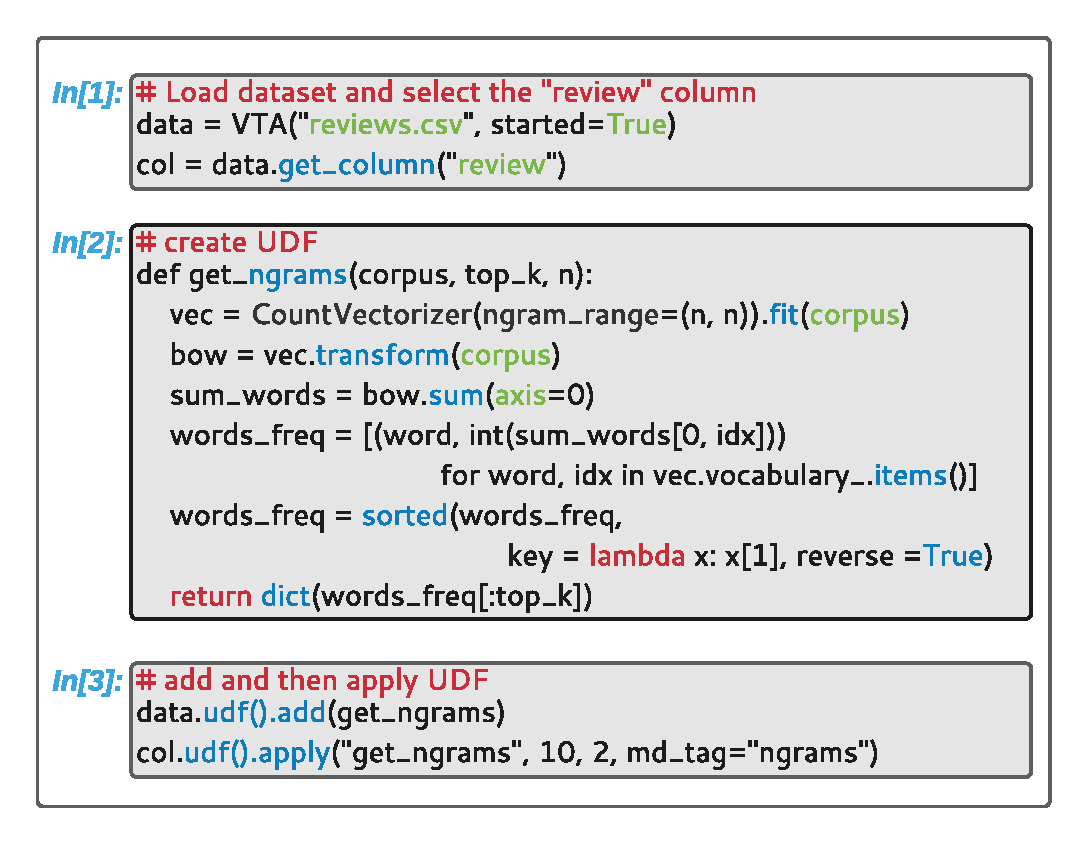
\includegraphics[width=\linewidth]{figures/udfs.pdf}
  \caption{\small  Example of adding a user-defined function (UDF) as a new operator and then applying the operator. The example UDF here computes the top $K$ $n$-grams of a given corpus. In general, \system enables users to create new operators by either composing (`piping') existing operators or specifying custom functions (UDFs).\label{fig:udf}} 
  %\vspace{-20pt}
\end{figure}



\subsubsection{Coordination operators}
The coordination operators in \vta are designed to enable coordination among views. We have enhanced the existing \vta implementation~\cite{rahman2020leam} so that users can dynamically add interactions to Data View and charts in Chart View. As show in Table~\ref{tab:operators}, there are two types of coordination operators: \code{internal} and \code{external}. The \code{internal} coordination operators allow users to set the selection type of an existing visualization---for example, setting the barchart selection from \emph{single} to \emph{multi} in Figure~\ref{fig:chartview_interact}. The \code{external} coordination operators allow users to enable coordination among views in \system. While the initial implementation of \vta supports only unidirectional coordination~\cite{rahman2020leam} (\emph{uni\_link} in Table~\ref{tab:operators}), \system supports bidirectional coordination using the \emph{bi\_link} operation. Once two views are linked by a bidirectional coordination, interacting with one visualization will update/modify the other visualization. For example, in Figure~\ref{fig:chartview_coordinate}, the barchart and scatterplot are linked via a bidirectional coordination. Therefore, selection a visualization mark (\ie bar or circle) in either updates the corresponding visualization. Moreover, \system also supports coordination of more than two views~\cite{rahman2020leam}. For example, adding a coordination between the barchart and Data View automatically links the scatterplot with the Data View (Figure~\ref{fig:chartview_coordinate_multi}). \system maintains a coordination graph to keep track of the linked views which we discuss in Section~\ref{sec:system}.

\begin{figure}[!htb] 
%  \vspace{-10pt}
  \centering
  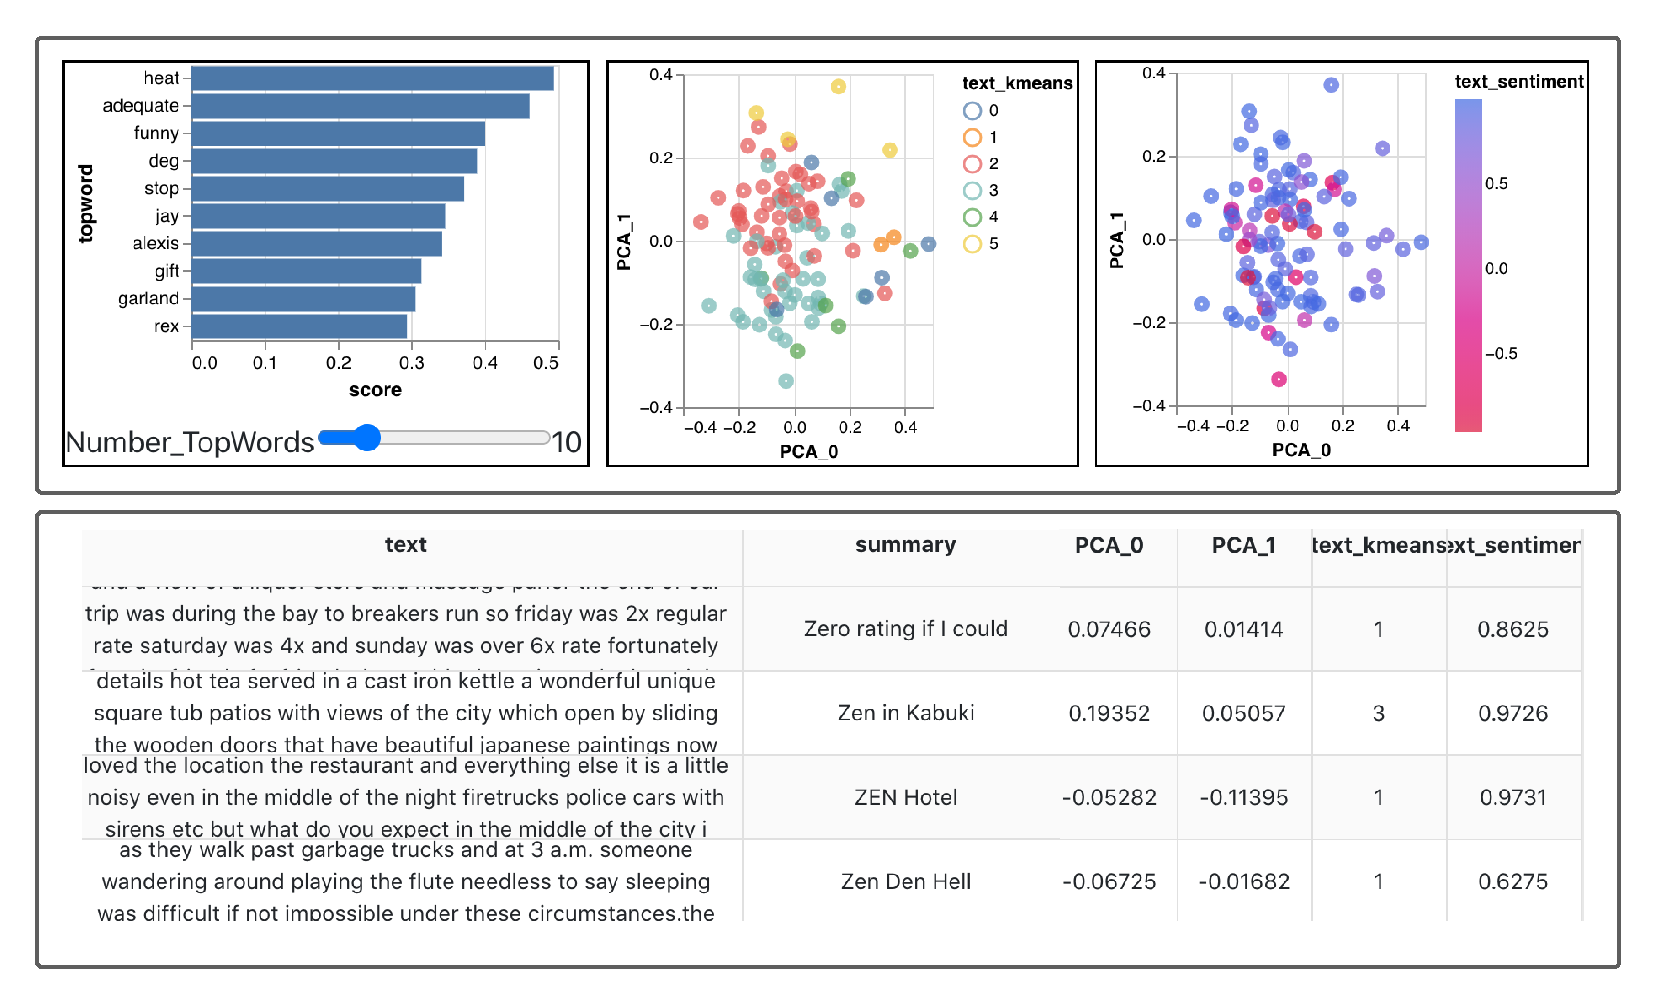
\includegraphics[width=\linewidth]{figures/chart_view.pdf}
  \caption{\small \todo{Draw figures} Example of dynamic coordination creation. The figure displays the barchart (generated in Figure~\ref{fig:chartview_interact}), a Scatterplot of reviews clustered using $k$-means clustering, and the corresponding data in Data View. To relate a word in the chart with reviews both in Data View and the scatterplot, the user issues a \vital command in Code Editor (see inset). Clicking a bar in the barchart filters reviews in Data View and highlights relevant reviews in the scatterplot. \label{fig:chartview_coordinate_multi}} 
  %\vspace{-20pt}
\end{figure}


\subsection{\vital: Declarative \vta Specification}
The JSON-style specifications for \vta introduced by Rahman et al.~\cite{rahman2020leam} can be difficult for the users to compose with advanced operations requiring multiple nested objects. Moreover, such specification format is quite different from popular scripting languages like R and Python that are widely used by analysts. Therefore, we have developed \vital, a python-based library for declaratively specifying \vta commands in Code Editor of \system. We show several examples of \vital commands that implement the \vta operators in Figure~\ref{fig:workflow} (\code{project}, \code{mutate}, \code{visualize}, \code{aggregate}), Figure~\ref{fig:chartview_interact} (\code{visualize}, \code{coordinate}), and Figure~\ref{fig:udf} (\code{udf}. All four \vta operator classes are packaged as a \code{VTA} class. To enable \vta operators on a dataset, users are required to instantiate a \code{VTA} object in Code Editor (see the first cell in Figure~\ref{fig:workflow} and~\ref{fig:udf}). The \vital commands are compiled and executed by the backend python runtime. \system employs a \emph{task queue} to manage the sequence of \vital commands written in the Code Editor (see Section~\ref{sec:system}). 
